\documentclass{report}
\usepackage[utf8]{inputenc}
\usepackage[T1]{fontenc}
\usepackage[frenchb]{babel}
\usepackage{amssymb}
\usepackage{mathtools}
\usepackage{listingsutf8}
\usepackage{verbatim}
\usepackage{xcolor}
\usepackage{graphicx}
\usepackage[toc,page]{appendix}

\lstloadlanguages{R}

\begin{document}
\lstset{
    language=R,
    basicstyle=\footnotesize,
    numbers=left,
    backgroundcolor=\color{white},
    breakatwhitespace=false,
    breaklines=true,
    captionpos=b,
    commentstyle=\color{green},
    extendedchars=true,
    keepspaces=true,
    keywordstyle=\bfseries\color{blue},
    numbersep=5pt,
    numberstyle=\tiny\color{gray},
    showtabs=false,
    stringstyle=\color{red},
    tabsize=2,
    title=\lstname
}

\title{SY09 - TP1}
\date{Mars 2016}
\author{Stéphane LOUIS et Paul GOUJON}
\pagenumbering{gobble}
\maketitle

\newpage
\tableofcontents{}

\newpage
\chapter{Avant propos}
\paragraph{Rapport}
Ce document présente les résultats que notre binôme a obtenu au cours du premier TP de SY09.

\paragraph{Annexes}
Nous vous invitons à consulter les annexes tout au long de votre lecture de ce rapport. Celles-ci contiennent certaines portions de code, expliquant comment nous avons obtenu certains de nos résultats.

\newpage
\pagenumbering{arabic}
\chapter{Le Racket du Tennis}


\section{Introduction}
Ce chapitre présente les résultats obtenus au cours de l'analyse d'un jeu de données recensant des paris effectués sur des matchs de Tennis de niveau international s'étant déroulés entre 2009 et 2015. Au cours de ses analyses, l'entreprise \textregistered LOUGOUJ s'est aperçu que certains résultats pouvaient laisser penser que des matchs avaient été truqués. Ce rapport à donc pour vocation d'exposer de manière objective l'analyse qui a été faite de ces données, et apporter quelques éléments de questionnement quant à l'irréprochabilité de certains joueurs.
\section{Format de données}
Les données sont fournies sous forme d'un data frame. Chaque ligne de ce dernier représente un pari effectué sur un match de Tennis, et chacune de ses colonnes contient une information différente le concernant. Les différents attributs dont nous disposons sur les paris sont les suivants.
\begin{itemize}
  \item \verb+match_book_uid+ : identifiant du pari
  \item \verb+match_uid+ : identifiant du match
  \item \verb+winner+ : identifiant du gagnant
  \item \verb+loser+ : identifiant du perdant
  \item \verb+book+ : identifiant du bookmaker
  \item \verb+year+ : année du match
  \item \verb+odds_winner_open+ : côte du futur vainqueur au début du match
  \item \verb+odds_winner_close+ : côte du futur vainqueur à la fin du match
  \item \verb+odds_loser_open+ : côte du futur perdant au début du match
  \item \verb+odds_loser_close+ : côte du futur perdant à la fin du match
  \item \verb+implied_prob_winner_open+ : probabilité induite de gain du match par le futur gagnant au début du match
  \item \verb+implied_prob_winner_close+ : probabilité induite de gain du match par le futur gagnant à la fin du match
  \item \verb+implied_prob_loser_open+ : probabilité induite de gain du match par le futur perdant au début du match
  \item \verb+implied prob_loser_close+ : probabilité induite de gain du match par le futur perdant à la fin du match
  \item \verb+moved_towards_winner+ : variable indiquant si les côtes ont évolué en faveur du joueur qui a remporté le match
\end{itemize}

\section{Analyse descriptive générale}
\paragraph{Statistiques générales}
Dans un premier temps, nous nous intéressons aux statistiques descriptives générales de l'échantillon.
\begin{table}[h!]
	\centering
	\caption{Statistiques descriptives générales}
	\label{tab:table1}
	\begin{tabular}{c|c}
   		Année de début & 2009\\
   		\hline
   		Année de fin & 2015\\
  		\hline
  		Nombre de matchs & 25993\\
  		\hline
  		Nombre de paris & 126461\\
  		\hline
  		Nombre de joueurs de tennis & 1523\\
      \hline
      Nombre de bookmakers & 7\\
      \hline
      Moyenne de paris par matchs & 4.766358
	\end{tabular}
\end{table}

\section{Analyse approfondie orientée joueurs}
\subsection{Données générales : joueurs et matchs}
\paragraph{Joueurs}
Nous nous intéressons dans un premier temps au nombre de joueurs, et la proportion d'etre eux ayant gagné ou perdu au moins un match. Donnons par le suite les valeurs concernant le nombre de matchs par joueur.
\begin{table}[h!]
	\centering
    \caption{Gagnants, perdants, joueurs}
	\label{tab:table2}
	\begin{tabular}{c|c}
   		Nombre de joueurs ayant gagné au moins un match & 899 \\
   		\hline
   		Nombre de joueurs ayant perdu au moins un match & 1502 \\
  		\hline
  		Nombre total de joueurs & 1523 \\
	\end{tabular}
\end{table}
\begin{table}[h!]
	\centering
	\caption{Nombre de matchs par joueur}
	\label{tab:table3}
	\begin{tabular}{c|c|c|c}
        Matchs & Gagnés & Perdus & Joués\\
   		\hline
   	    Min & 0 & 0 & 0\\
   		\hline
   	    Max & 447 & 190 & 527\\
   		\hline
   	    Mean & 17.02227 & 17.02227 & 34.04453
	\end{tabular}
\end{table}
\subsection{Histogramme présentant la répartition des joueurs en fonction de
leur proportion de victoires}
\paragraph{Introduction}
Afin de représenter les performances des joueurs, nous avons trouvé intéressant
de dessiner un histogramme représentant la répartition des joueurs en fonction
de leur proportion de victoire par rapport au nombre de matchs qu'ils ont joué.
\begin{center}
    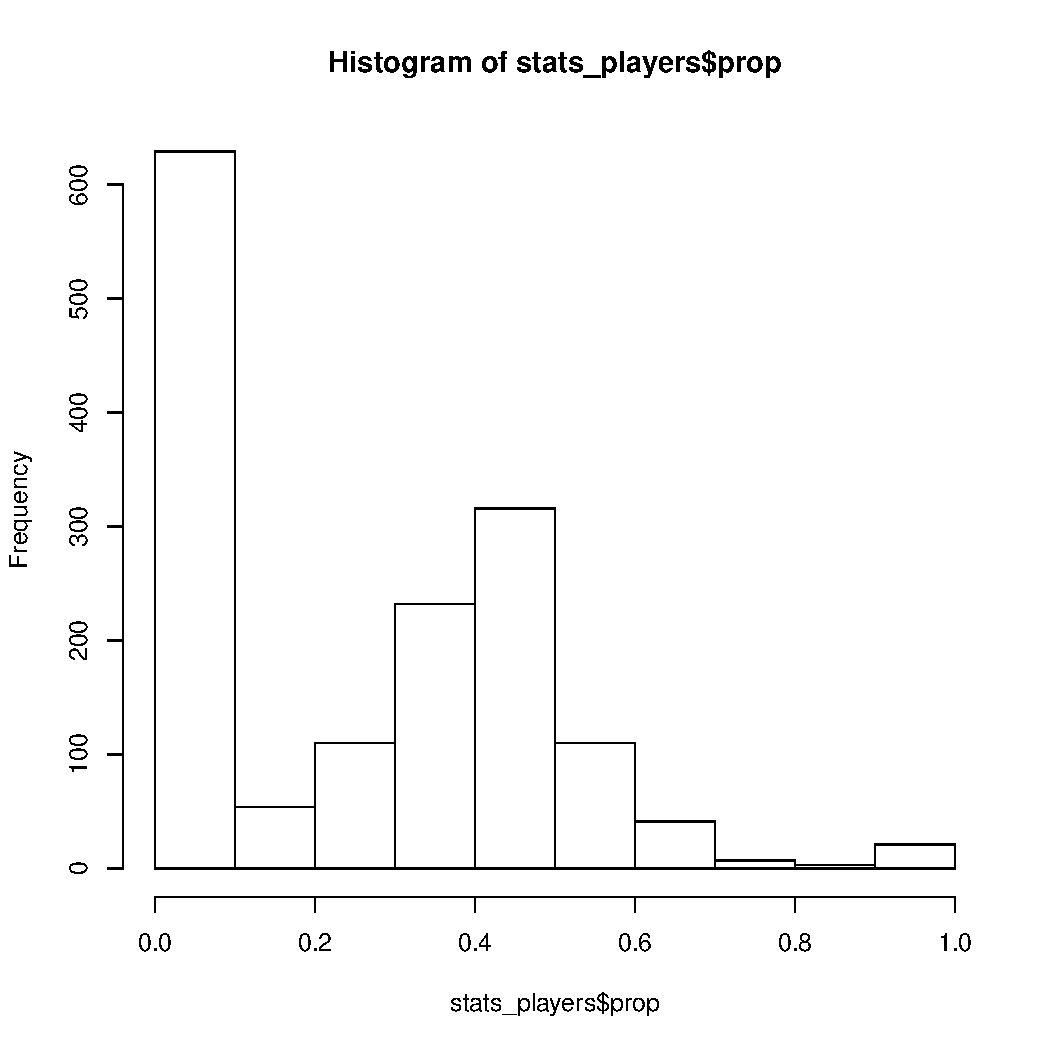
\includegraphics[width=\textwidth]{hist.pdf}
\end{center}
\paragraph{Interprétation}
Cet histogramme met en exergue un nombre important de joueur n'ayant eu aucune
victoire ou n'ayant eu que très peu de victoires au cours d'un très faible nombre de matchs. On voit ensuite une répartition plutôt intuitive, montrant qu'une
majorité de joueurs a obtenu une proportion de victoire entre 40 et 60\% (probablement la partie de l'histogramme la plus représentative, comprenant l'ensemble des joueurs ayant joué un nombre suffisant de matchs pour que la statistique soit significative). Pour
finir, nous pouvons expliquer le léger pic final de notre histogramme par le
fait qu'un certain nombre de joueurs n'a joué qu'un très faible nombre de matchs, et ainsi potentiellement obtenu
une grand nombre de victoire comparé au nombre de défaites.

\section{Matchs Truqués}
\subsection{Introduction}
\paragraph{Objectif}
L'objectif de cette section est de mettre en avant certains matchs dits
"suspects", c'est à dire présentant une évolution de probabilité de défaite (ou
de victoire) supérieure à 0.1 en
valeur absolue en faveur de l'un ou l'autre des joueurs.
\paragraph{Data frame de travail}
De la même manière qu'auparavant, nous commençons par restreindre notre data frame de paris à un data frame de matchs uniques et le trions.
\subsection{Répartition des probabilités initiales de victoire des futurs gagnants}
\paragraph{Diagramme en boite à moustache}
Nous trouvions intéressant de vous présenter la répartition des probabilités de
victoire des futurs gagnants en début de match au sein d'un diagramme en boite à moustache.
\begin{figure}[h!]
\begin{center}
    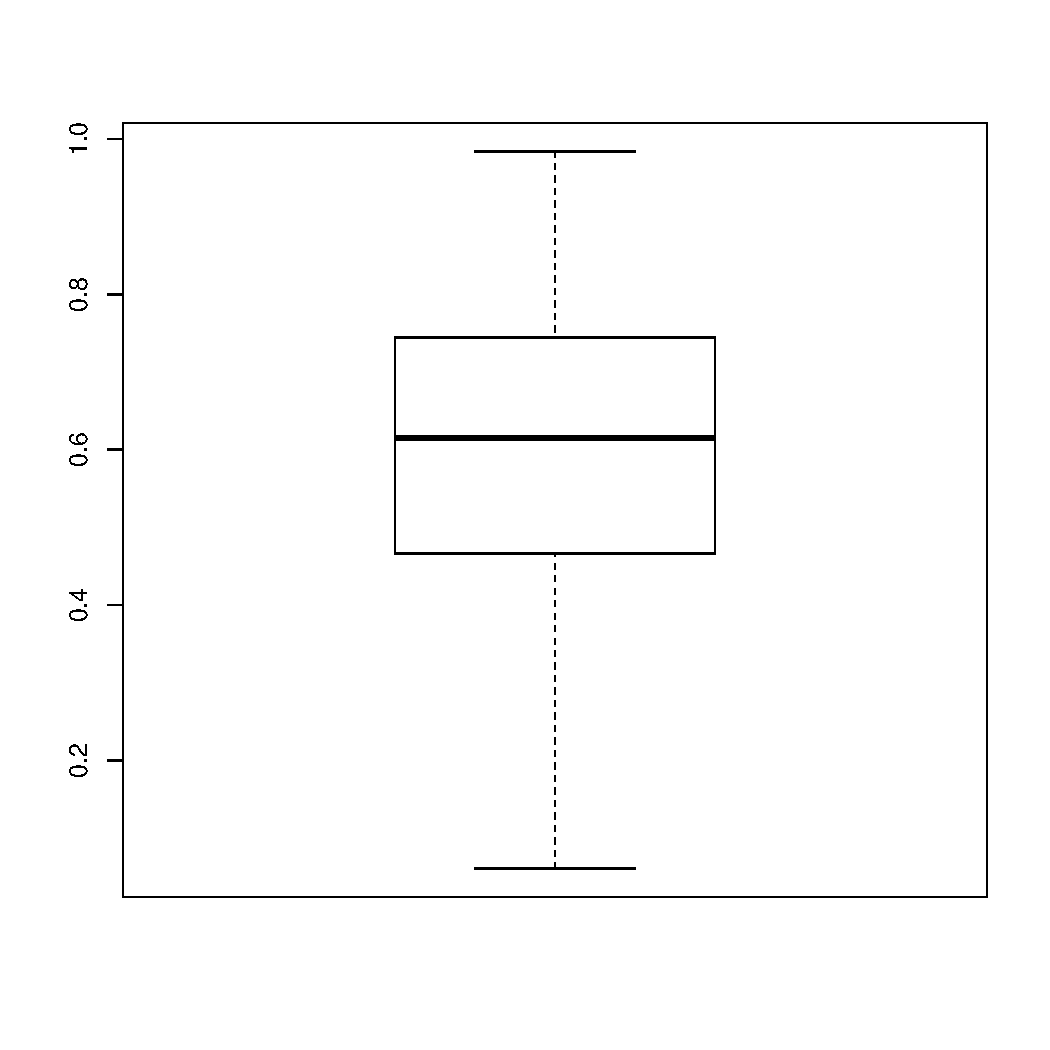
\includegraphics[width=0.6\textwidth]{boxplot2.pdf}
    \caption{Répartition des probabilités induites initiales de victoire des joueurs}
\end{center}
\end{figure}
\paragraph{Interprétation}
Encore une fois, ce diagramme est assez intuitif : il est normal que la
majorité des joueurs de l'échantillon aient une probabilité de victoire initiale
comprise entre 0.4 et 0.6 étant donné que la majorité des matchs que nous
étudions sont des matchs représentatifs, donc suffisamment équilibrés. Notons
tout de même quelques valeurs extrêmes traduisant probablement le fait que
quelques matchs sont hautement déséquilibrés.
\subsection{Matchs suspects}
\paragraph{Détermination des matchs dits suspects}
Nous nous intéressons maintenant à l'ensemble des matchs présentant une évolution
de probabilité de défaite d'un des joueurs supérieure à 0.1. Nous ajoutons donc à notre data frame une colonne contenant la valeur absolue de la
différence entre les probabilités induites de victoire du futur perdant en début et fin de
match. Nous séléctionnons ensuite au sein d'un deuxième data frame les matchs
dont la probabilité a évolué de plus de 0.1, et les comptons.
\paragraph{Résultats}
De l'étude de ces matchs suspects, nous tirons les statistiques suivantes:
\begin{table}[h!]
  \centering
  \caption{Matchs suspects}
  \label{tab:table4}
  \begin{tabular}{c|c}
        Nombre de matchs suspects & 1497\\
      \hline
        Idem avec mouvement de probabilité en faveur du gagnant & 949\\
      \hline
        Nombre de joueurs impliqués dans au moins un match suspect & 495\\
      \hline
        Idem avec mouvement de probabilité en faveur du gagnant & 413
  \end{tabular}
\end{table}
\paragraph{Caractérisation des matchs}
Telles que nous sont fournies les données, il n'est pas aisé de "caractériser"
les matchs truqués. Nous avons cependant pensé à deux méthodes qui pourraient
faire émerger des caractéristiques communes:
\begin{itemize}
\item Représenter la proportion de matchs truqués par rapport au nombre de
    matchs joués, par année, afin de voir si la plupart des malversations ont eu
    lieu la même année.
\item Représenter la proportion de matchs truqués en fonction du niveau des
    joueurs (son pourcentage de victoire), afin de savoir à quel niveau le tennis mondial
    est touché.
\end{itemize}
\subsection{Bookmakers concernés}
\paragraph{Tous les bookmakers sont ils concernés ?}
Nous souhaitons par la suite savoir si tous les bookmakers sont concernés par ce
phénomène de matchs truqués. Nous étudions donc tous les uniques bookmakers
présents dans ce data frame de matchs suspects.
\paragraph{Résultat}
Le résultat est encore plus suspect : seuls 4 bookmarkers sur 7 sont concernés
par ce phénomène d'évolution de probabilité. Les bookmakers suspects sont les suivants : \verb+A, B, C et D+
\subsection{Joueurs suspects}
\paragraph{Détermination des joueurs suspects}
Pour finir, nous souhaitons faire émerger une liste de joueurs impliqués dans les matchs suspects. Nous considérons un joueur comme \verb+"suspect"+ s'il a perdu au moins 10 matchs suspects et
\verb+"hautement suspect"+ s'il a perdu au moins 10 matchs suspects avec évolution de probabilité en faveur du gagnant. Il est en effet plus facile d'influencer l'issue d'un match en le perdant qu'en le gagnant.
\begin{table}[h!]
  \centering
  \resizebox{0.75\textwidth}{!}{\begin{minipage}{\textwidth}
  \caption{Détermination des joueurs suspects}
  \label{tab:table4}
  \begin{center}\begin{tabular}{c|c|c}
    Joueur & suspect & hautement suspect\\
    \hline
    0c638adbb5 & 14 & -\\
    \hline
    a9362aae6f & 11 & -\\
    \hline
    0ffe23c8b8 & 14 & 10\\
    \hline
    dd83d74956 & 11 & -\\
    \hline
    1a798648b6 & 10 & -\\
    \hline
    716e5cafc4 & 11 & -\\
    \hline
    69f958da99 & 11 & -\\
    \hline
    3e74a4acf8 & 12 & -\\
    \hline
    e998255367 & 13 & 10\\
    \hline
    290a3dce64 & 14 & -\\
    \hline
    194dbaf338 & 10 & -\\
    \hline
    b24990a981 & 15 & 11\\
    \hline
    01870a94b6 & 12 & -\\
    \hline
    879bac1da6 & 10 & -\\
    \hline
    8d028ece8a & 18 & 14\\
    \hline
    f16cc81d23 & 12 & 10\\
    \hline
    b7080834c4 & 15 & -\\
    \hline
    7cd9b31cde & 10 & -\\
    \hline
    163a93c4de & 14 & -\\
    \hline
    6bb26867a0 & 11 & -\\
    \hline
    d5e122c7e9 & 13 & -\\
    \hline
    4f7f8e1b43 & 12 & -\\
    \hline
    b084b94a57 & 14 & -\\
    \hline
    be7c4f5126 & 10 & -\\
    \hline
    c169137b1c & 10 & -\\
    \hline
    69a1209d7f & 15 & -\\
    \hline
    afd6124804 & 10 & -\\
    \hline
    c9d4889bac & 14 & 11\\
    \hline
    614c204988 & 10 & -\\
    \hline
    45df519812 & 13 & -\\
    \hline
    7f4c89750c & 14 & -\\
    \hline
    9c92af8ca1 & 11 & -\\
    \hline
    33367d2147 & 11 & -\\
    \hline
    822130a312 & 12 & -\\
    \hline
    6a4a7e0a92 & 12 & -\\
    \hline\hline
    Totaux\\
    \hline
    35 & 429 & 99
    \end{tabular}
    \end{center}
    \end{minipage}}
\end{table}

\newpage
\chapter{Crabs - Première partie}


\section{Analyse du jeu de données "Crabs"}

\subsection{Introduction}

\subsection{Analyse descriptive des données}
\paragraph{Caractérisation des données}
Nous disposons, dans ce jeu de données sur les crabes, des caractéristiques suivantes :
\begin{itemize}
\item sp : espèce
\item sex : sexe
\item index : un numéro entre 1 et 50 qui représente un crabe dans un groupe
\item FL, RW, CL, CW, BD : des mesures de caractéristiques morphologiques
\end{itemize}
\paragraph{Taille de l'échantillon}
Il y a un total de 200 crabes, 100 de chaque espèce et, pour chaque espèce, 50
mâles et 50 femelles.
\paragraph{Analyse descriptive de l'échantillon}
Nous effectuons un première analyse descriptive de la population, qui produit les résultats suivants.
\begin{table}[h!]
  \centering
  \caption{Analyse descriptive de la population}
  \label{tab:table4}
  \begin{tabular}{c|c|c|c|c|c}
    Attribut & FL & RW & CL & CW & BD\\
    \hline
    Minimum & 7.20 & 6.50 & 14.70 & 17.10 & 6.10\\
    \hline
    1er Quartile & 12.90 & 11.00 & 27.27 & 31.50 & 11.40\\
    \hline
    Mediane & 15.55 & 12.80 & 32.10 & 36.80 & 13.90\\
    \hline
    Moyenne & 15.58 & 12.74 & 32.11 & 36.41 & 14.03\\
    \hline
    3e Quartile & 18.05 & 14.30 & 37.23 & 42.00 & 16.60\\
    \hline
    Maximum & 23.10 & 20.20 & 47.60 & 54.60 & 21.60
  \end{tabular}
\end{table}
\begin{figure}[h!]
\begin{center}
    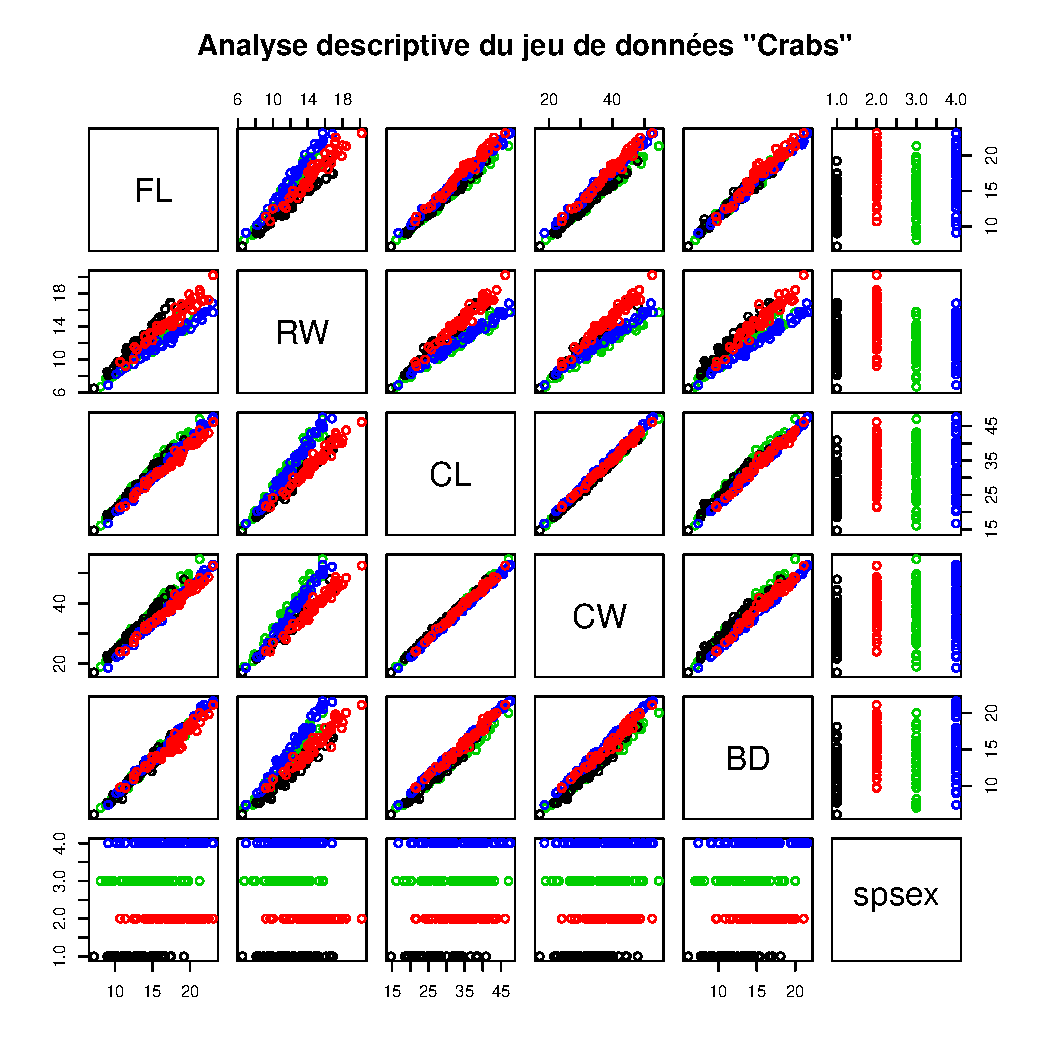
\includegraphics[width=\textwidth]{plotcrabsp1.pdf}
    \caption{Pair plot représentant les caractéristiques morphologiques des individus de la population}
\end{center}
\end{figure}
\paragraph{Légende}
\begin{itemize}
\item Noir : Bleu.Feminin
\item Rouge : Orange.Feminin
\item Vert : Bleu.Masculin
\item Bleu : Orange.Masculin
\end{itemize}
\paragraph{Interprétation}
A première vue, il n’existe pas de différence morphologique selon l’espèce ou le
sexe. Les valeurs des mesures de caractéristiques morphologiques des crabes ne
permettent ni une identification du sexe, ni une identification de l’espèce du
crabe en question.
\newpage
\subsection{Corrélation}
\paragraph{Etude de la corrélation des variables}
Nous cherchons maintenant à déterminer le degré de corrélation entre les différentes variables. La matrice de corrélation entre les variables quantitatives est la suivante.
\begin{center}
$\begin{pmatrix}
    cor(X,Y) & FL & RW & CL & CW & BD\\
    FL & 1.00\\
    RW & 0.91 & 1.00 \\
    CL & 0.98 & 0.89 & 1.00\\
    CW & 0.96 & 0.90 & 1.00 & 1.00\\
    BD & 0.99 & 0.89 & 0.98 & 0.97 & 1.00
\end{pmatrix}$
\end{center}
\paragraph{Interprétation}
Nous constatons que la corrélation entre les différentes variable est très importante.
Nous expliquons cela par le fait que la taille globale d'un
crabe influe fortement sur chacune de ses caractéristiques physionomiques.
\paragraph{Proposition de traitement}
Pour une meilleure visualisation il faudrait réussir à s'affranchir de cette influence qu'a la taille d'un crabe sur ses caractéristique (chose que nous tenterons de faire au sein de la seconde étude du jeu de données concernant les crabes, dans le chapitre 4 de notre rapport).

\newpage
\chapter{Analyse des Composantes Principales (ACP) }


\section{ACP}
\subsection{Introduction}
\paragraph{Objectif}
L'objectif de ce chapitre est d'appliquer les notions théorique de l'Analyse de
Composantes Principales vues en cours de SY09.
\paragraph{Prérequis}
Nous disposons du jeu de données suivant
\begin{center}
$M = \begin{pmatrix}
    3 & 4 & 3 \\
    1 & 4 & 3 \\
    2 & 3 & 6 \\
    4 & 1 & 2
\end{pmatrix}$
\end{center}
Les individus sont tous pondérés de la même manière et $\mathbb{R}^p$ est munit de
la métrique euclidienne.
\subsection {Axes factoriels et pourcentages d'inertie expliquée}
\paragraph{Axes factoriels et inertie expliquée}
Nous souhaitons dans un premier temps calculer les axes factoriels du nuage
ainsi définis ainsi que les pourcentages d'inertie expliquée par chacun de ces
axes.
\paragraph{Centrage des données}
L'ACP se fait sur des données centrées. Nous centrons donc notre échantillon.
\begin{center}
$Mc = \begin{pmatrix}
    0.5 & 1 & -0.5\\
    -1.5 & 1 & -0.5\\
    -0.5 & 0 & 2.5\\
    1.5 & -2 & -1.5
\end{pmatrix}$
\end{center}
\paragraph{Matrice de variance}
Souhaitons par la suite calculer la matrice de variance du nuage.
Elle se calcule selon la formule:
\begin{equation}
V = Mc^T * Dp * Mc
\end{equation}
Avec Dp la matrice diagonale pondérée par l'effectif (souvent appelée "métrique
des poids").
\begin{equation}
Dp = (1/n) * I_n
\end{equation}
Nous obtenons :
\begin{center}
$V = \begin{pmatrix}
    1.25\\
    -1 & 1.5\\
    -0.75 & 0.5 & 2.25 \\
\end{pmatrix}$
\end{center}
Puis nous utilisons la fonction eigen(V) pour obtenir les vecteurs et valeurs
propres de la matrice de variance.
\paragraph{Valeurs propres}
\begin{itemize}
\item $\lambda1 = 3.1988922$
\item $\lambda2 = 1.4684861$
\item $\lambda3 = 0.3326217$
\end{itemize}
\paragraph{Vecteurs propres}
\begin{equation}
u1 =
\begin{pmatrix}
    0.5240424\\
    -0.5093555\\
    -0.6825955
\end{pmatrix}
\end{equation}
\begin{equation}
u2 =
\begin{pmatrix}
    0.3386197\\
    -0.6107855\\
    0.7157358
\end{pmatrix}
\end{equation}
\begin{equation}
u3 =
\begin{pmatrix}
    0.7814834\\
    0.6062161\\
    0.1475997
\end{pmatrix}
\end{equation}
\paragraph{Pourcentage d'inertie expliquée}
L'inertie expliquée totale du nuage est égale à la somme des valeurs propres de la matrice de variance, soit 5. Il suffit pour connaitre le pourcentage d'inertie expliquée par un axe factoriel de calculer le rapport entre sa valeur propre, et la valeur propre totale. Ainsi, le pourcentage d'inertie expliquée pour chaque axe factoriel est respectivement de 64\%, 30\% et 6\% environ.
\subsection{Calcul des composantes principales}
\paragraph{Théorie}
La matrice des composantes principales s'obtient selon la formule:
\begin{equation}
C = Mc * U
\end{equation}
Avec U la matrice des vecteurs propres.
\paragraph{Matrice des composantes principales}
Nous obtenons la matrice des composantes principales suivante:
\begin{center}
    $\begin{pmatrix}
        0.09396341 & -0.7993436 & 0.92315798\\
        -0.95412132 & -1.4765829 & -0.63980885\\
        -1.96850984 & 1.6200297 & -0.02174241\\
        2.82866775 & 0.6558968 & -0.26160672
    \end{pmatrix}$
\end{center}
\paragraph{Représentation des individus}
Nous obtenons la représentation des
individus dans le premier plan factoriel en utilisant les deux premières
composantes principales (c'est à dire les composantes de l'échantillon selon les
deux premiers axes factoriels).
\begin{figure}[h!]
\begin{center}
    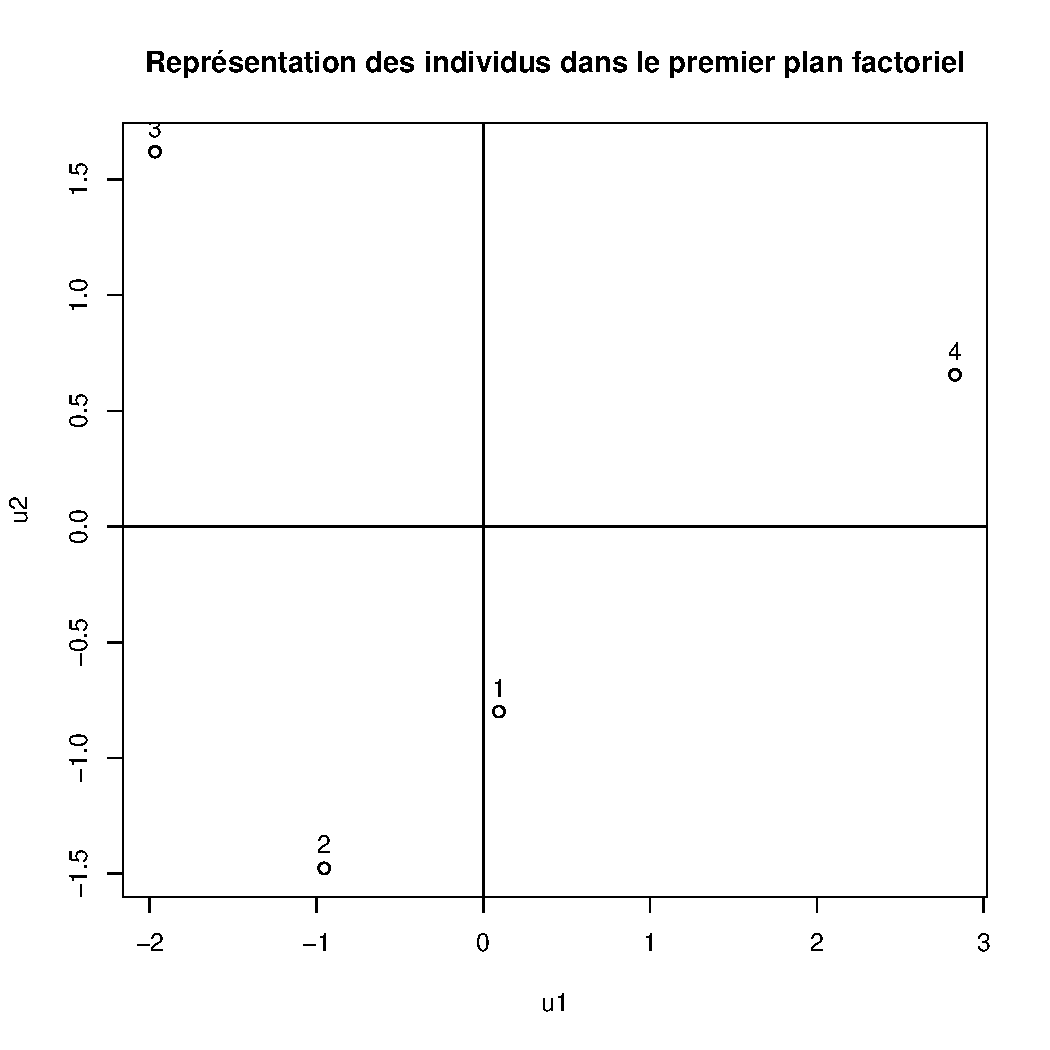
\includegraphics[width=\textwidth]{acpq3ok.pdf}
    \caption{Représentation des individus dans le premier plan factoriel}
\end{center}
\end{figure}
\subsection{Représentation des variables}
\paragraph{Réalisation}
Nous représentons également les variables dans le premier plan factoriel.
\begin{figure}[h!]
\begin{center}
    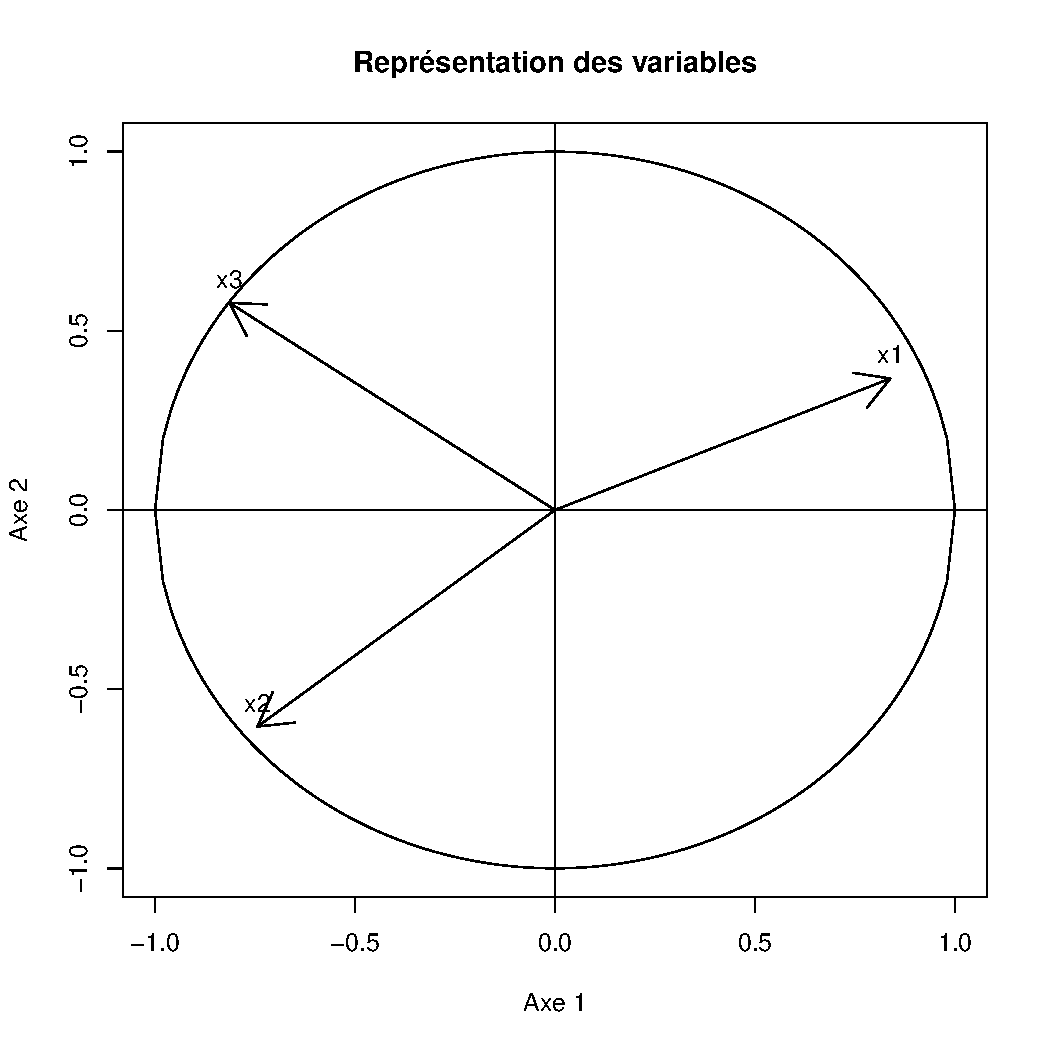
\includegraphics[width=\textwidth]{reprvar.pdf}
    \caption{Représentation des variables dans le premier plan factoriel}
\end{center}
\end{figure}
\subsection{Calcul de la somme de la multiplication des composantes
principales par les vecteurs propres (Formule de reconstitution)}
\paragraph{Formule}
Nous sommes maintenant amenés à étudier la formule suivante :
Cette formule correspond à la formule de reconstitution du cours.
\begin{equation}
R = \sum_{k=1}^n c_\alpha * u'_\alpha
\end{equation}
\paragraph{Calcul}
Calculons R pour chaque valeur de k.
\paragraph{k = 1}
\begin{center}
    $R = \begin{pmatrix}
        0.04924081 & -0.04786078 & -0.0641390\\
        -0.50000000 & 0.48598695 & 0.6512789\\
        -1.03158256 & 1.00267132 & 1.3436959\\
        1.48234175 & -1.44079748 & -1.9308358
    \end{pmatrix}$
\end{center}
\paragraph{k = 2}
\begin{center}
    $R = \begin{pmatrix}
        -0.2214326 & 0.4403667 & -0.6362579\\
        -1.0000000 & 1.3878624 & -0.4055644\\
        -0.4830087 & 0.0131806 & 2.5032092\\
        1.7044413 & -1.8414098 & -1.4613869
    \end{pmatrix}$
\end{center}
\paragraph{k = 3}
\begin{center}
    $R = \begin{pmatrix}
        0.5 & 1.0 & -0.5\\
        -1.5 & 1.0 & 0.5\\
        -0.5 & 0.0 & 2.5\\
        1.5 & -2.0 & -1.5
    \end{pmatrix}$
\end{center}
\paragraph{Interprétation}
La formule ci-dessus est en réalité la formule de reconstitution. Lorsque k = 3, nous obtenons la reconstitution de la matrice initiale. En dessous de k = 3, les matrices obtenues sont des approximations de la matrice initiale, n'incorporant qu'une fraction de l'information initiale. Cette propriété est parfois utilisée pour compresser des données lorsque l'on est prêt à perdre un peu d'information.

\newpage
\chapter{Crabs - Seconde Partie}

\section{Introduction}
\paragraph{Introduction}
Au cours de cette seconde partie de l'étude du jeu de données "Crabs", nous souhaitons
utiliser les fonctions natives de R pour effectuer une ACP. Nous nous familiarisons avec ces outils sur un premier dataset (celui étudié en cours), puis appliquons cela au dataset "Crabs".
\paragraph{Objectif}
Notre objectif est de mettre en évidence des différences morphologiques entre les différentes espèces de crabes, et en fonction de leur sexe.

\section{Utilisation des outils R}
\subsection{Présentation des fonctions}
\paragraph{Introduction}
Dans un premier temps, nous appliquons les fonctions natives de R sur le data frame du cours afin d'essayer d'obtenir les mêmes résultats, et discutons les fonctions en question.
\paragraph{princomp}
La fonction \verb+princomp+ réalise l'ACP du data frame que nous lui fournissons et retourne le résultat sous la forme d'un objet \verb+princomp+. Lorsque l'on appelle cet objet au sein de la console R, sont affichées les écarts types de chacune des composantes de l'échantillon.
\paragraph{summary}
L'appel à la fonction \verb+summary+ sur l'objet \verb+princomp+ nous affiche différentes informations nous permettant de juger l'importance de chacune des composantes, notamment leurs écarts-types, leurs inerties expliquées ainsi que l'inertie expliquée cumulée.
\paragraph{loadings}
Pour finir, l'appel à la fonction \verb+loadings+ sur l'objet \verb+princomp+ nous sert principalement à prendre connaissance des vecteurs propres de la matrice de covariance, c'est à dire les axes factoriels.
\subsection{Fonctions d'affichage}
\paragraph{Introduction}
Nous nous intéressons maintenant aux fonctions d'affichage de R appliquées à l'objet \verb+princomp+ et leurs paramètres.
\paragraph{plot}
La fonction plot affiche un histogramme représentant l'inertie expliquée par chacune des composantes.
\begin{figure}[h!]
\begin{center}
    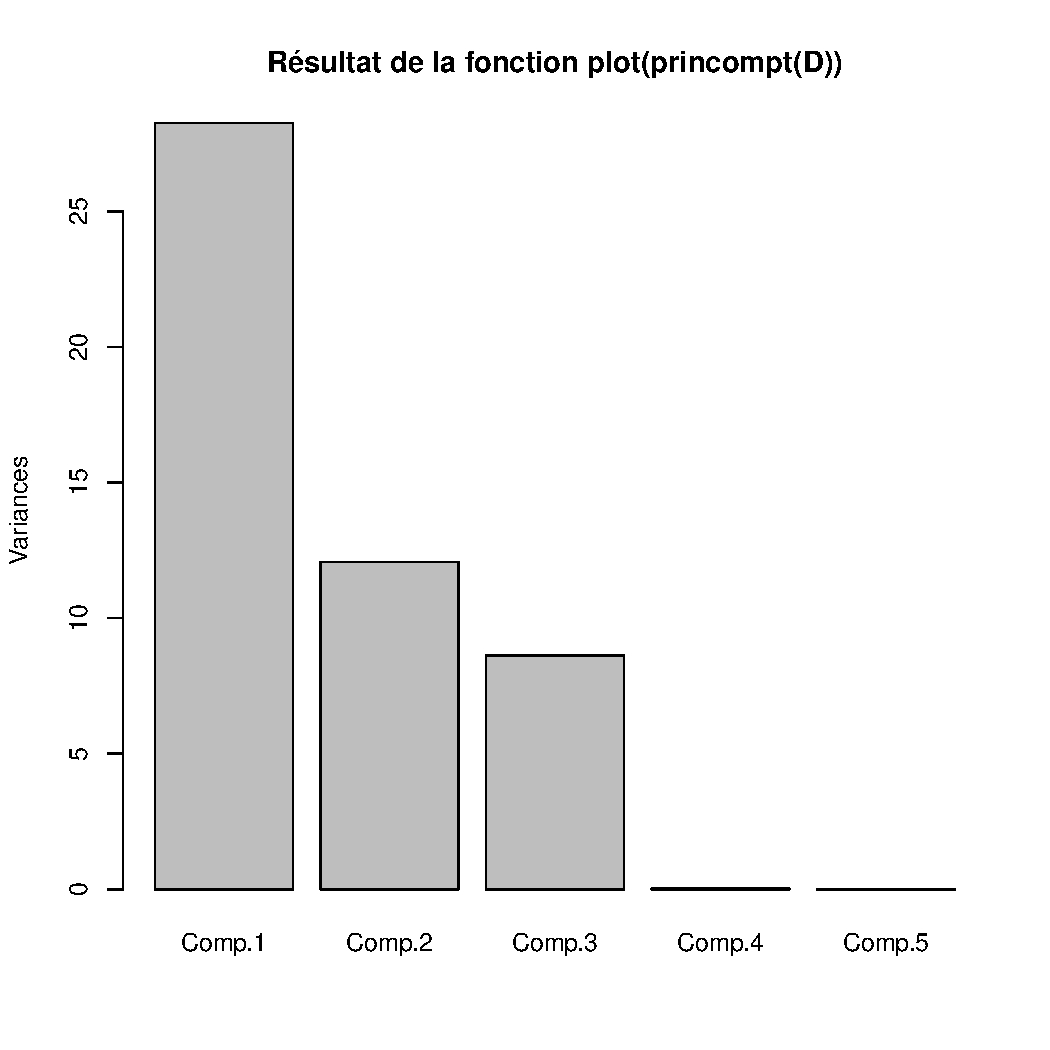
\includegraphics[width=\textwidth]{e4q1.pdf}
    \caption{Résultat de la fonction plot(princomp(D)) avec D le data frame étudié}
\end{center}
\end{figure}
\paragraph{biplot}
La fonction biplot affiche les individus et les variables sur le premier plan factoriel.
\begin{figure}[h!]
\begin{center}
    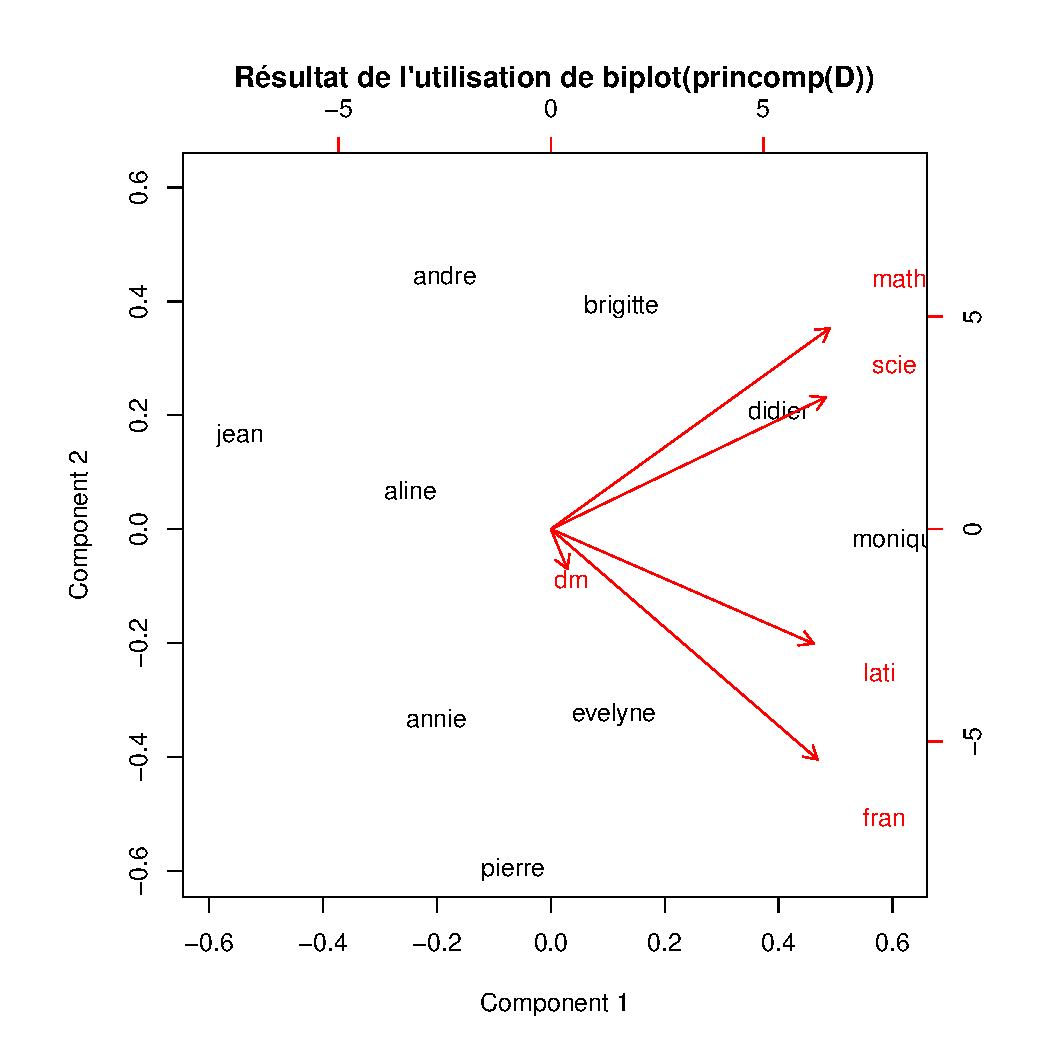
\includegraphics[width=\textwidth]{biplot1.pdf}
    \caption{Résultat de la fonction biplot(princomp(D)) avec D le data frame étudié}
\end{center}
\end{figure}
\paragraph{Paramètres de biplot}
La fonction biplot prend en paramètre différents arguments modifiant la représentation des individus :
\begin{itemize}
\item \verb+biplot(princompt(D), c(1,3))+ : Affiche les individus et variable sur les axes factoriels venant des composantes 1 et 3
\item Un paramètre \verb+scale+ permet de modifier l'échelle de l'une ou l'autre des composantes. Par défaut, l'échelle des variables est égale à $\lambda^{scale}$, et les observations $\lambda^{n-1}$, ou $\lambda$ sont les valeurs singulières des calculs effectués par princomp.
\item Un dernier paramètre, en lien avec le précédent, initialise $\lambda$ à 1 pour le calcul de l'échelle, et l'échelle des variables est montante et égale à \verb+sqrt(n)+, celle des observations est descendante et également égale à \verb+sqrt(n)+
\end{itemize}
\paragraph{Exemple de biplot selon les axes factoriels 1 et 3}
L'étude de la représentation des individus selon les axes factoriels déduits des composantes 1 et 3 nous prouve que la représentation obtenue à partir des axes factoriels déduits des composantes 1 et 2 étaient décrivait avec beaucoup plus d'exactitude notre population.
\begin{figure}[h!]
\begin{center}
    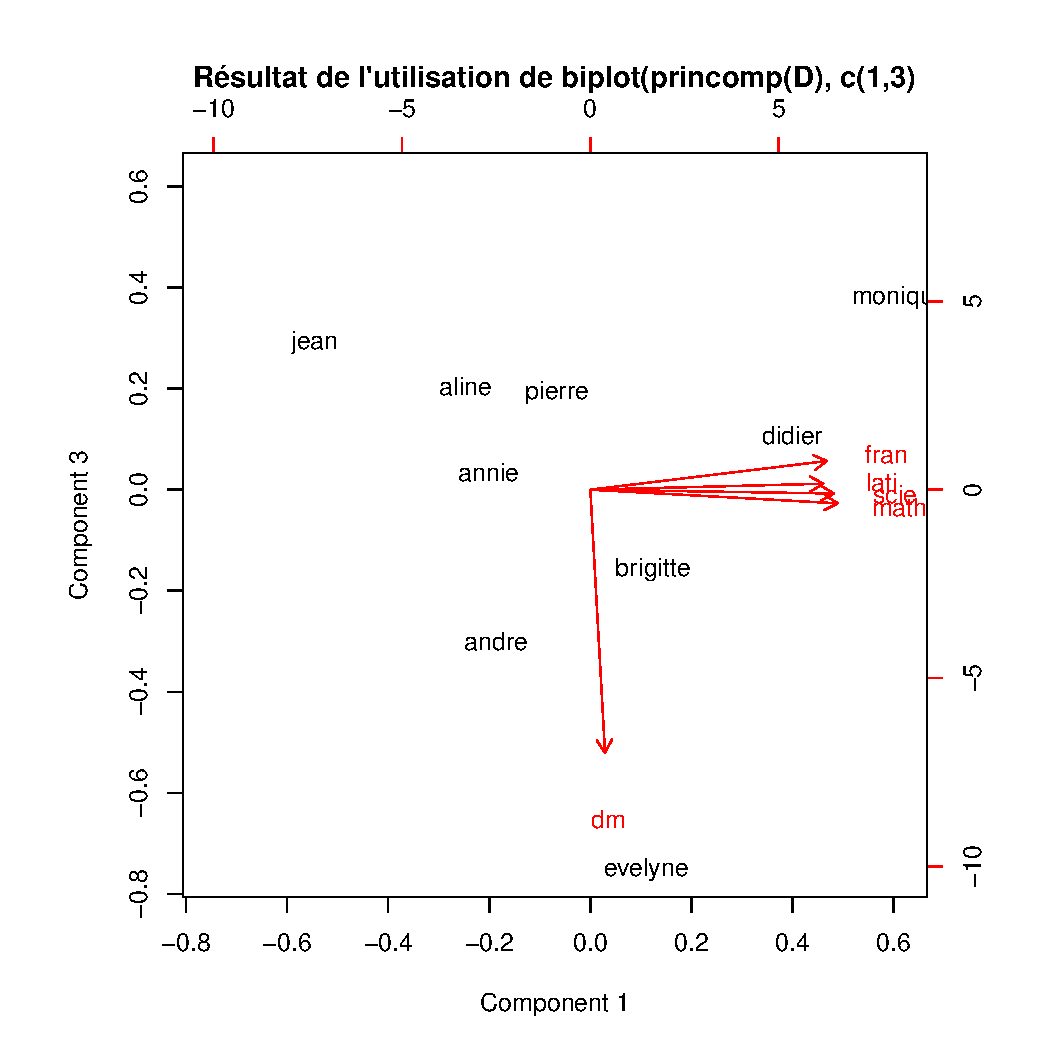
\includegraphics[width=\textwidth]{biplot2.pdf}
    \caption{Résultat de la fonction biplot(princomp(D), c(1,3)) avec D le data frame étudié}
\end{center}
\end{figure}

\section{Nouvelle étude du jeu de données "Crabs"}
\subsection{Introduction}
\paragraph{Introduction}
Nous allons au sein de cette section effectuer une nouvelle étude du jeu de données "Crabs", en utilisants les outils de R découverts précédemment, nous permettant d'effectuer une ACP. Nous étudierons dans un premier temps le jeu de données sans prétraitement, puis dans un second temps essaierons d'améliorer la qualité de notre représentation en testant deux méthodes.
\subsection{Analyse sans prétraitement}
\paragraph{ACP via R sur le jeu "Crabs"}
A l'aide de la fonction princomp, il est fort agréable d'obtenir instantanément les valeurs suivantes.
\begin{figure}[h!]
\begin{center}
    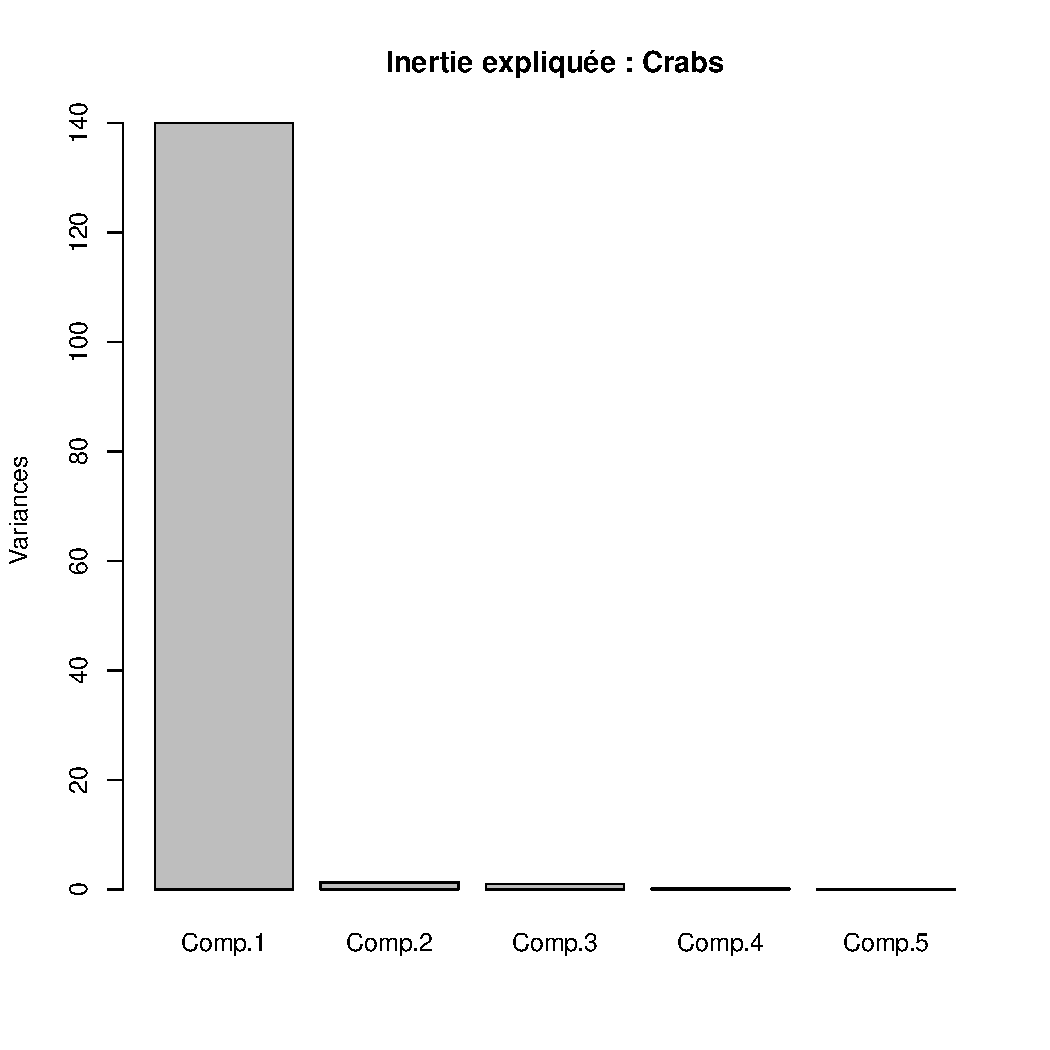
\includegraphics[width=0.9\textwidth]{plotcrabs.pdf}
    \caption{Répartition de l'inertie expliquée pour l'ACP sur le jeu "Crabs"}
\end{center}
\end{figure}
\newpage
Après avoir représenté la répartition d'inertie expliquée par les différentes composantes, voici la représentation des individus et variables dans le premier plan factoriel.
\begin{figure}[h!]
\begin{center}
    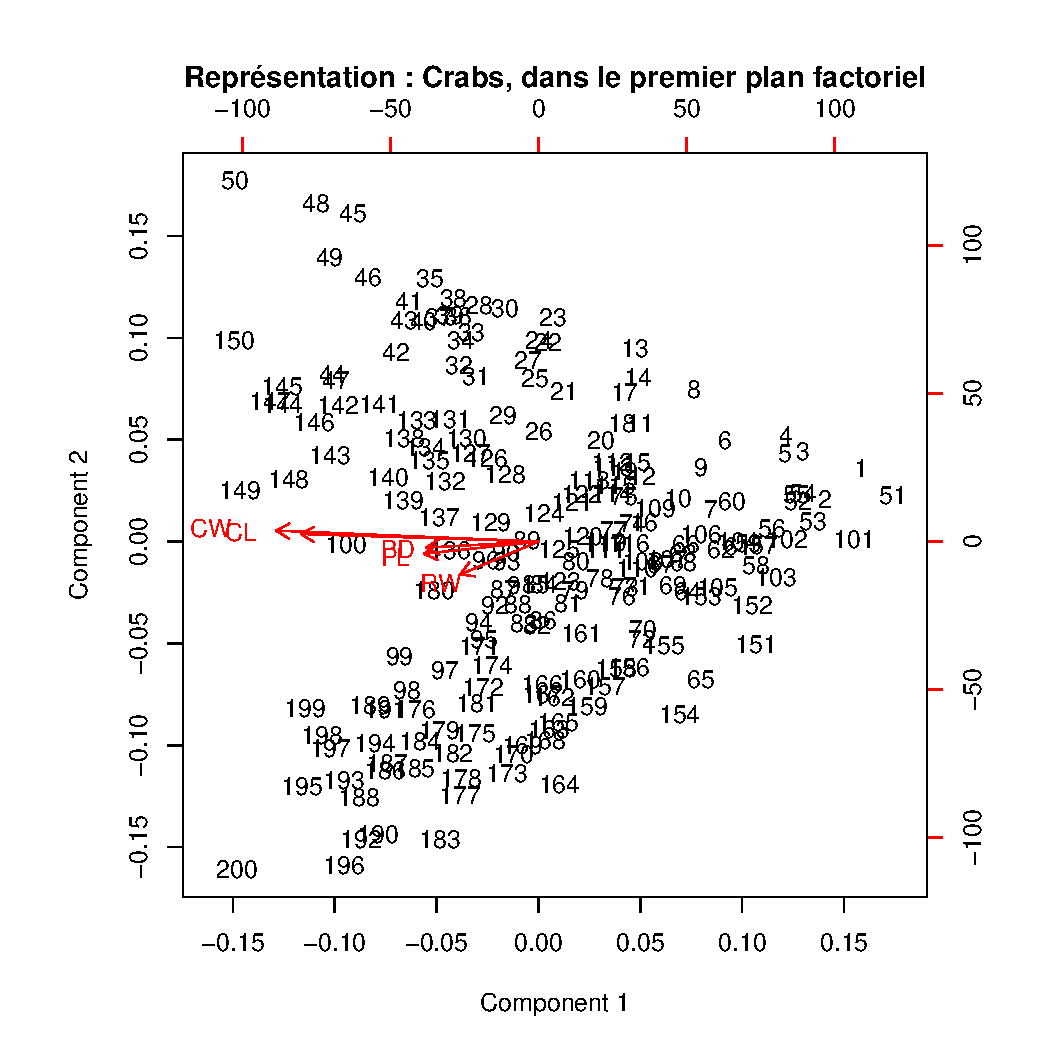
\includegraphics[width=0.9\textwidth]{biplotcrabs.pdf}
    \caption{Représentation des individus et variables du jeu "Crabs" dans le premier plan factoriel}
\end{center}
\end{figure}
\paragraph{Interprétation}
Comme nous l'avions vu au sein de la première étude du jeu de données "Crabs", il est très difficile de différencier les crabes en fonction de leur espèces ou de leur sexe. Cela est dû au fait que les différentes variables morphologiques sont très corrélées.
\subsection{Analyse avec prétraitement}
\paragraph{Introduction}
Nous décidons d'essayer deux méthodes pour améliorer la qualité de la représentation. Nous allons dans un premier temps essayer de simplifier les populations en les étudiant par leur moyenne. Notre seconde tentative consiste à essayer de "gommer" l'influence de la taille globale des crabes dans sur les variables morphologiques en les divisant par la somme de la taille de tous les membres de l'individu, pour chaque individu.
\paragraph{Simplification par la moyenne}
La première méthode que nous avons tentée a été de simplifier l'échantillon en effectuant la même étude que précédemment, mais cette fois sur les moyennes de chaque population (male orange, femelle orange, male bleu, femelle bleu). Notre motivation principale était de réduire le nombre de points sur notre représentation afin d'en améliorer la lisibilité.
Nous obtenons la représentation suivante.
\begin{figure}[h!]
\begin{center}
    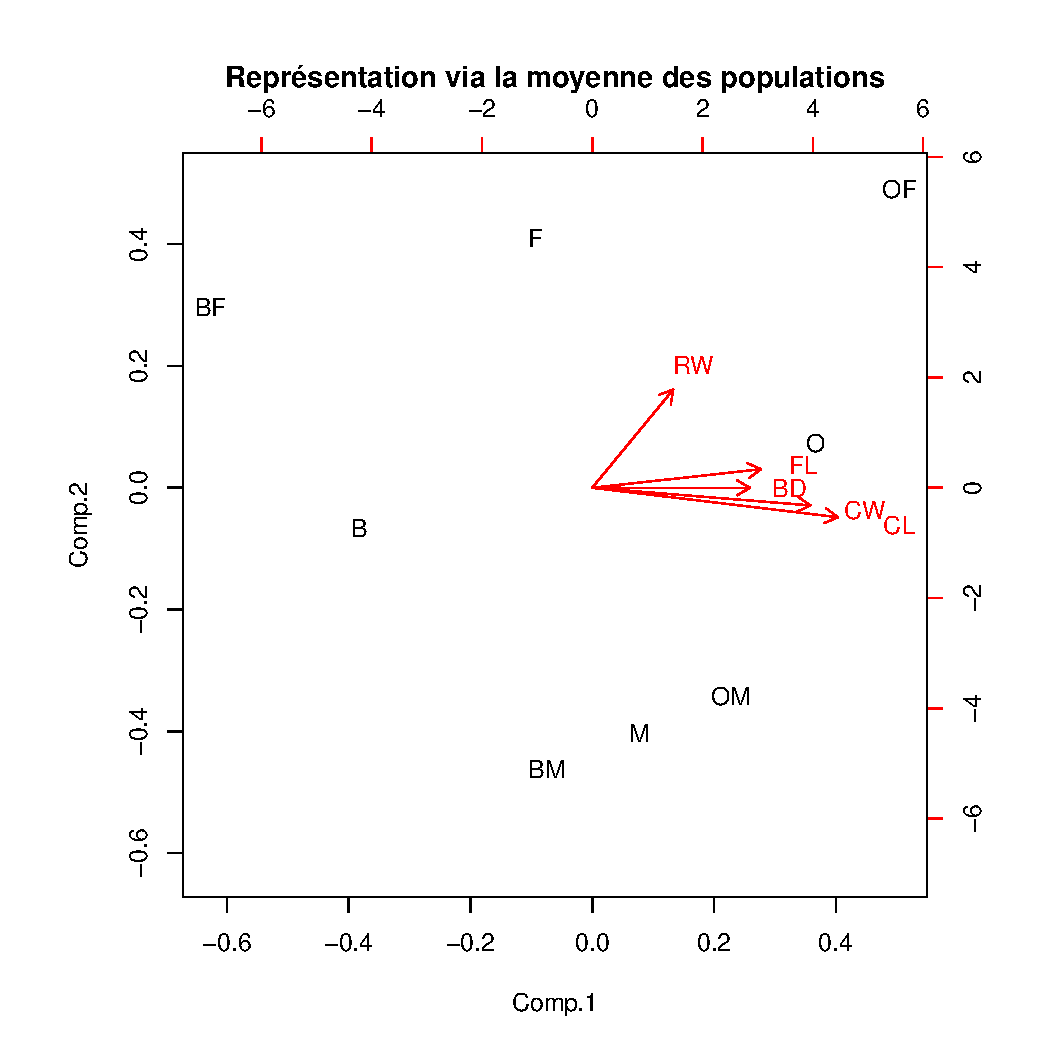
\includegraphics[width=0.9\textwidth]{crabsmean.pdf}
    \caption{Représentation par la moyenne de chaque population}
\end{center}
\end{figure}
\paragraph{Interprétation}
Il semblerait, selon cette représentation, que les crabes femelles aient une tendance à avoir un membre arrière plus large que celui des mâles. Il semblerait également que les crabes oranges aient tendance à être plus petits que les crabes bleus.
\paragraph{"Gommage du facteur taille"}
La seconde méthode que nous avons tentée nous est venue en nous renseignant sur la manière d'essayer de restreindre l'influence qu'a la taille globale du crabe sur ses caractéristiques morphologiques. Pour y arriver, il suffit en fait de faire le rapport entre chacune des caractéristiques morphologique du crabe et sa taille globale (soit la somme de la taille de chacun de ses membres). La représentation en résultant permet une bien meilleure représentation des caractéristiques de chaque espèce et chaque sexe.
\begin{figure}[h!]
\begin{center}
    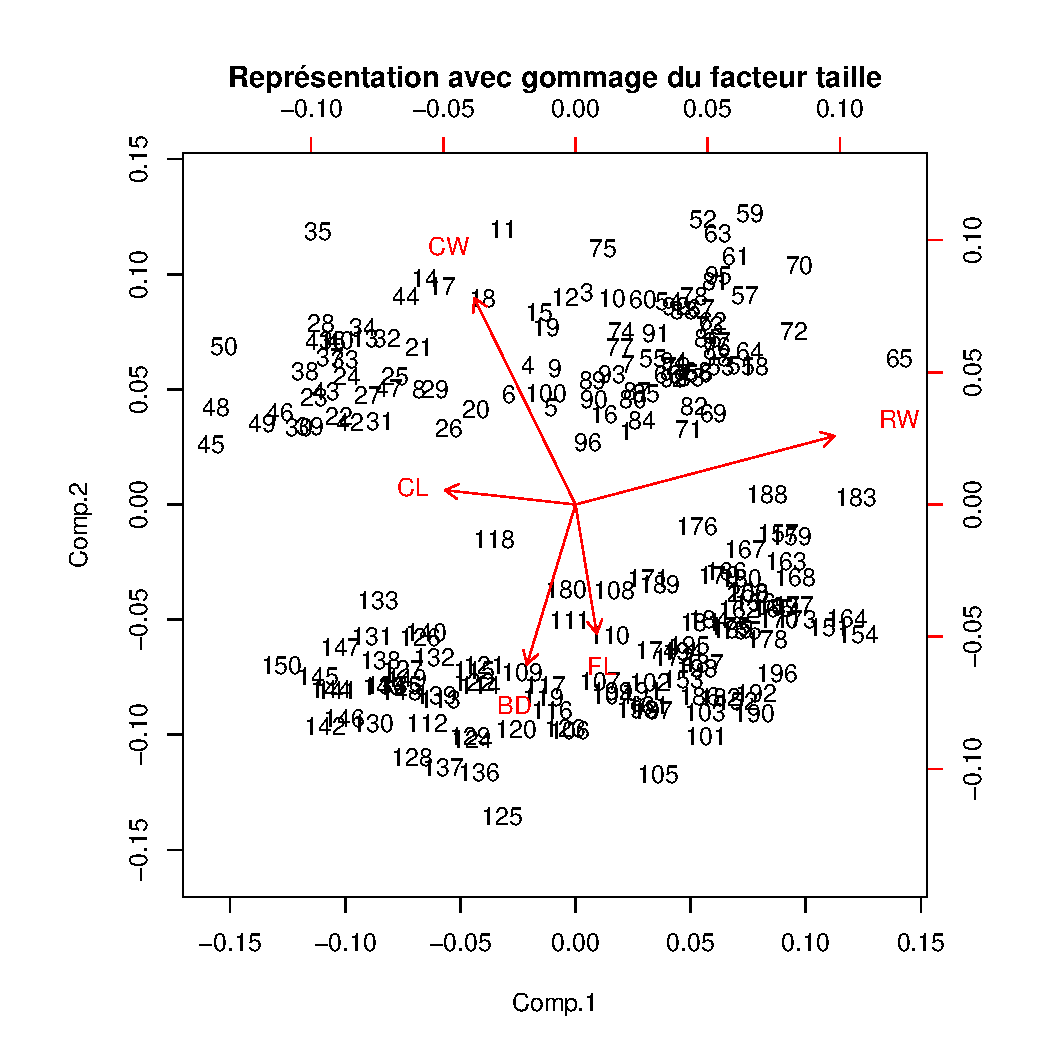
\includegraphics[width=0.9\textwidth]{newcrabs.pdf}
    \caption{Représentation avec "gommage" de la taille des crabes}
\end{center}
\end{figure}
\paragraph{Interprétation}
En utilisant cette représentation, il devient évident que les femelles ont tendance à avoir un membre arrière plus développé que celui des mâles. Cependant, un critère de différenciation supplémentaire émerge permettant de faire la différence entre les deux espèces : il semblerait que la carapace des crabes bleus ait tendance à être plus développée que celle des crabes oranges, tandis que les crabes orange ont un lobe frontal et une profondeur de corp plus important que les crabes bleus.
\paragraph{Avec des couleurs c'est souvent mieux...}
L'utilisation de la représentation colorée est nécessaire pour faire la correspondance entre points et espèces / sexe.
\begin{figure}[h!]
\begin{center}
    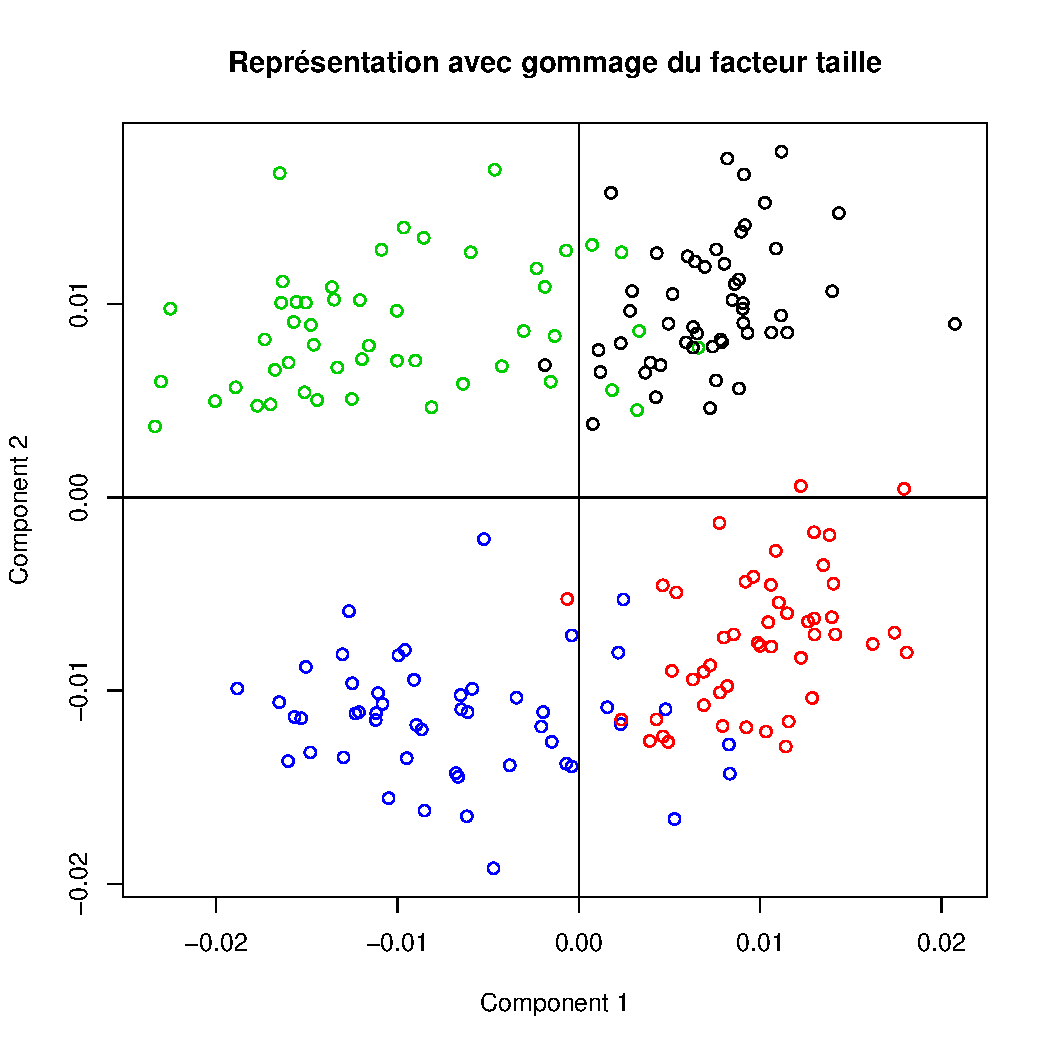
\includegraphics[width=0.9\textwidth]{newcrabs2.pdf}
    \caption{Autre représentation avec "gommage" de la taille des crabes}
\end{center}
\end{figure}
\paragraph{Légende}
\begin{itemize}
\item Noir : Bleu.Feminin
\item Rouge : Orange.Feminin
\item Vert : Bleu.Masculin
\item Bleu : Orange.Masculin
\end{itemize}

\newpage
\chapter{Conclusion}
\paragraph{Conclusion}
Ce premier TP sur R a été l'occasion d'effectuer un bon premier tour d'horizon de la puissance de R. Dans un premier temps nous avons découvert les fonctions de base de R. Nous avons ensuite abordé le concept d'analyse exploratoire des données, souvent précédée et suivie par du traitement de données, afin de les rendre significatives. Dans une seconde partie de TP nous avons pu aborder un première méthode d'analyse des données : l'Analyse en Composantes Principales. Cela a été l'occasion pour nous d'appliquer ces concepts vus en cours au travers d'un exercice théorique et deux exercices pratiques. Pour finir, au sein des deux grandes parties de ce TP (étude des matchs de Tennis et étude des Crabs), nous avons été encouragés à approfondir, et ainsi, "prendre notre envol" dans le domaine de l'analyse de donnée \& data mining.

\paragraph{Note}
Notons aussi le douloureux mais utile apprentissage du langage \LaTeX !

\newpage
\begin{appendices}
\chapter{Introduction}
\paragraph{Avant propos}
Les annexes de ce rapport de TP contiennent principalement des morceaux de code nous ayant permis d'obtenir les différents résultats présentés tout au long du rapport. Ne seront développés que les parties nous semblant pertinentes. Il ne nous semblait pas nécessaire de ré-expliquer le fonctionnement de fonctions basiques de R.

\chapter{Le Racket du Tennis}
\section{Analyse descriptive générale}
\subsection{Analyses descriptive générale} %====================================
\paragraph{Méthode}
Ces résultats sont obtenus en utilisant les méthodes de base de R sur le data
frame.
\paragraph{Nombre moyen de paris par match}
Nous pouvons obtenir le nombre de paris par match en construisant une table de
contingence sur les \verb+match_uid+ présents dans ce data frame de paris. Il
suffit ensuite de calculer la moyenne de la colonne représentant le nombre de
paris en fonction du match pour obtenir le nombre moyen de paris par match.
\begin{lstlisting}
# Construction de la table de contigence
> con_paris = table(books.sel$match_uid)
> mean(con_paris)
\end{lstlisting} %==============================================================

\subsection{Analyse approfondie orientée joueurs} %=============================
\paragraph{Méthode}
Nous restreignons dans une premier temps notre data frame à un certain nombre
d'uniques matchs, puis analysons ce "subset".
\paragraph{Matchs uniques}
Obtenir un subset de notre data frame initial ne contenant que des matchs
uniques (c'est à dire une instance par match, au lieu de x paris par match)
revient à demander à R de créer un nouveau data frame, et ne sélectionner que
des matchs non dupliqués à partir du data frame initial.
\begin{lstlisting}
> matchs = books.sel[which(!duplicated(books.sel$match_uid)),]
\end{lstlisting}
Afin d'éviter que tout problème d'ordonancement des données ne vienne fausser
nos analyses, nous appliquons immédiatement une fonction de tri au data frame
ainsi créé.
\begin{lstlisting}
> matchs = matchs[sort.int(as.character(matchs$match_uid), index.return=T)$ix,]
\end{lstlisting}
\paragraph{Matchs gagnés / perdus}
Pour étudier par la suite les statistiques de matchs gagnés et perdus, il suffit
de réutiliser le concept de tables de contingences abordé pour la première fois
au sein de la section précédente.
\begin{lstlisting}
> con_win = table(matchs$winner)
> max(con_win)
> min(con_win)
> mean(con_win)
\end{lstlisting}
\paragraph{Matchs joués}
Le data frame en l'état ne nous permet pas d'obtenir facilement des statistiques
concernant le nombre de matchs joués par joueurs. Heureusement, le web (toile
d'araignée en français) nous renseigne sur la manière de "merger" deux tables de
contingences. Dans un premier temps nous sommons le nombre de victoire et de
défaites pour chaque joueur, afin d'obtenir le nombre de matchs joués.
\begin{lstlisting}
> con_played = c(con_win, con_los)
> con_played = tapply(con_played, names(con_played), sum)
\end{lstlisting}
Nous obtenons une table de contingence contenant le nombre de matchs joués en
fonction de l'identifiant du joueur. Nous pouvons ainsi appliquer les fonctions
de maximum, minimum et moyenne à cette table. %=================================

\subsection{Histogramme} %======================================================
\paragraph{Méthode}
Etant relativement débutant en R, nous ne connaissions aucun moyen d'exploiter
les tables de contingences, de manière à obtenir une troisième table de
contingence contenant le rapport Nombre de victoires / Nombre de matchs
joués des joueurs. Nous avons donc décidé d'essayer d'utiliser une autre
méthode pour obtenir cette statistique.
\paragraph{Subsetting le data frame initial}
Nous ne sommes, pour cette section, intéressé que par les statistiques de
concernant le nombre de victoires et de défaites de chaque joueur. Nous décidons
donc de garder uniquement les identifiants de booking, les identifiants de
match, les winners et les losers.
\begin{lstlisting}
> books_players = subset(books.sel, select=c("match_book_uid", "match_uid",
"winner", "loser"))
\end{lstlisting}
\paragraph{Matchs uniques}
Comme précédemment, nous ne gardons que les matchs uniques et les trions.
\begin{lstlisting}
> matchs_players = books_players[which(!duplicated(books_players$match_uid)),]
> matchs_players = matchs_players[sort.int(as.character(matchs$match_uid),
index.return=T)$ix,]
\end{lstlisting}
\paragraph{Aggrégations}
Nous aggrégeons par la suite dans deux data frames le nombre de matchs gagnés et
perdus par joueur. Puis nous appliquons de nouveau notre fonction de tri pour être
sûr de ne pas perdre l'ordre de nos données.
\begin{lstlisting}
> won_matchs = aggregate(match_uid ~ winner, matchs_players, function(x)
length(unique(x)))
> lost_matchs = aggregate(match_uid ~ loser, matchs_players, function(x)
length(unique(x)))
> won_matchs = won_matchs[sort.int(as.character(won_matchs$match_uid),
index.return=T)$ix,]
> lost_matchs = lost_matchs[sort.int(as.character(lost_matchs$match_uid),
index.return=T)$ix,]
\end{lstlisting}
\paragraph{Merge de data frames}
Nous souhaitons ensuite merger nos deux data frames en un seul. Nous voulons que
ce merge se fasse par identifiant de match. Nous devons donc renommer les
attributs de nos deux data frames \verb+won_matchs+ et \verb+lost_matchs+, qui
contiennent jusque là, rappelons le, les identifiants des joueurs sous le nom
\verb+winner+ ou \verb+loser+ et le nombre de victoires ou défaites par joueur
sous le nom \verb+match_uid+.
\begin{lstlisting}
> names(won_matchs)[names(won_matchs) == "match_uid"] = "nb_win"
> names(won_matchs)[names(won_matchs) == "winner"] = "identifier"
> names(lost_matchs)[names(lost_matchs) == "match_uid"] = "nb_los"
> names(lost_matchs)[names(lost_matchs) == "loser"] = "identifier"
> stats_players = merge(won_matchs, lost_matchs, by="identifier", all=T)
> str(stats_players)
'data.frame':   1523 obs. of  3 variables:
 $ identifier: Factor w/ 1527 levels "47c51695d6","cf2dc97a01",..: 1 2 3 4 5 6 7
 8 9 10 ...
 $ nb_win    : int  25 236 247 173 71 26 141 145 100 17 ...
 $ nb_los    : int  21 115 144 148 70 42 130 163 161 25 ...
\end{lstlisting}
\paragraph{Note}
Vous l'aurez noté, nous utilisons l'argument \verb+all=T+ afin de faire en
sorte que les valeurs \verb+NA+ soient aussi mergées : en effet, nos data frames
\verb+won_matchs+ et \verb+lost_matchs+ contiennent chacun 1523 levels, mais la
valeur \verb+NA+ pour, par exemple, les joueurs n'ayant pas gagné de match pour
l'un, ou encore les joueurs n'ayant pas perdu de match pour l'autre. Sans
l'utilisation de \verb+all=T+, tout level contenant un \verb+NA+ d'un côté comme
de l'autre n'aurait pas été mergé.
\paragraph{Traitement des NA}
Nous remplaçons donc ces NA par des 0 (et retrions nos données: on est jamais
trop prudents).
\begin{lstlisting}
> stats_players[is.na(stats_players)] = 0
> stats_players = stats_players[sort.int(as.character(stats_players$identifier),
index.return=T)$ix,]
\end{lstlisting}
\paragraph{Calcul du total de matchs joués par joueur}
Nous ajoutons ensuite une nouvelle colonne à notre data frame, correspondant au
total de matchs joués par joueur, soit la somme des matchs gagnés et perdus par
chaque joueur.
\begin{lstlisting}
> stats_players$total = stats_players$nb_win + stats_players$nb_los
> max(stats_players$total)
[1] 527
\end{lstlisting}
\paragraph{Note}
Nous retrouvons la valeur calculée auparavant... rassurant.
\paragraph{Proportion de victoires}
Nous atteignons enfin notre but, en ajoutant une dernière colonne à notre data
frame, correspondant à la proportion de victoires par joueur.
\begin{lstlisting}
> stats_players$prop = stats_players$nb_win / stats_players$total
> str(stats_players)
'data.frame':   1523 obs. of  5 variables:
 $ identifier: Factor w/ 1527 levels "47c51695d6","cf2dc97a01",..: 550 1315 1387
 637 461 817 652 527 47 127 ...
  $ nb_win    : num  1 0 0 12 22 1 16 4 92 30 ...
  $ nb_los    : num  3 1 1 11 31 2 12 5 96 57 ...
  $ total     : num  4 1 1 23 53 3 28 9 188 87 ...
  $ prop      : num  0.25 0 0 0.522 0.415 ...
\end{lstlisting}
\paragraph{Autocritique}
Tout au long de l'élaboration de cet histogramme, nous avons tenté d'être les
plus rigoureux possible. Cependant, notre méconnaissance du langage R nous a
très probablement fait commettre un certain nombre d'erreurs et contraint
d'utiliser certaines méthodes qui pourraient être décrites comme des
"workarounds", au lieu de pleinement utiliser la puissance de R.

Note à posteriori : Nous avons découvert très récemment que les tables de
contigences pouvaient être castées en data frames... et donc devenir ainsi
beaucoup plus faciles à manipuler. Si nous avions utilisé cela plus tôt, notre
résolution de cette question en aurait été grandement simplifiée. %=============

\subsection{Matchs truqués}
\paragraph{Méthode}
De la même manière que précédemment, nous subsettons notre data frame initial pour obtenir un data frame de matchs uniques. Par suite nous ajoutons une colonne à ce data frame égale à la valeur absolue de la différence entre la probabilité induite initiale de victoire du perdant en début de match et en fin de match. A partir de là, nous créons deux data frames subsets de notre data frame de matchs, l'un comprennant tous les matchs avec évolution de probabilité de plus de 0.1, et l'autre avec à la fois évolution de probabilité de plus et 0.1 ET ayant évolué en faveur du futur gagnant. Il suffit ensuite de compter pour chacun d'entre eux le nombre de matchs, et le nombre d'unique perdants.
\begin{lstlisting} %============================================================
> matchs = books.sel[which(!duplicated(books.sel$match_uid)),]
> matchs = matchs[sort.int(as.character(matchs$match_uid), index.return=T)$ix,]
> matchs$evol = abs(matchs$implied_prob_winner_close -
matchs$implied_prob_winner_open)
> matchs$evol_los = abs(matchs$implied_prob_loser_open - matchs$implied_prob_loser_close)
> suspects2 = matchs[which(matchs$evol_los > 0.1),]
> length(unique(as.character(suspects2$match_uid)))
[1] 1497
> suspects3 = suspects2[which(suspects2$moved_towards_winner),]
> length(unique(suspects3$match_uid))
[1] 949
> length(unique(c(as.character(suspects2$winner), as.character(suspects2$loser))))
[1] 495
> length(unique(c(as.character(suspects3$winner), as.character(suspects3$loser))))
[1] 413
\end{lstlisting} %==============================================================

\subsection{Bookmakers concernés} %=============================================
\paragraph{Méthode}
Trouver les bookmakers concernés par un ou plusieurs matchs suspects revient à sélectionner les bookmakers uniques présents dans notre data frame de matchs suspects.
\begin{lstlisting}
> unique(as.character(suspects2$book))
[1] "B" "A" "D" "C"
> unique(as.character(suspects3$book))
[1] "B" "A" "D" "C"
\end{lstlisting} %==============================================================

\subsection{Joueurs suspects}
\paragraph{Méthode}
Les joueurs suspects se repèrent en construisant les tables de contingences des perdants des matchs suspects, puis en sélectionnant au sein de ces tables de contingences les joueurs ayant plus de n défaites suspectes.
\begin{lstlisting}
# Suspects
> hsus = table(suspects2$loser)
> hsus = as.data.frame(hsus)
> hsus[which(hsus$Freq>9),]
# Hautement suspects
> hhsus = table(suspects3$loser)
> hhsus = as.data.frame(hhsus)
> hhsus[which(hhsus$Freq>9),]
\end{lstlisting}

\newpage
\chapter{Crabs - Première partie}
\paragraph{Note}
Nous ne développerons pas cette partie, qui n'utilise pas de fonction réellement complexe de R.

\chapter{ACP - Exercice Théorique}
\paragraph{Note}
Nous ne développerons pas cette partie, étant donné qu'elle repose principalement l'application à la lettre des méthodes enseignées en cours et rappelées sur les supports pédagogiques du moodle.

\newpage
\chapter{Crabs - Seconde partie}
\section{Utilisation des outils R}
\paragraph{Note}
Nous ne développerons pas cette partie, étant donné qu'elle ne consiste qu'à utiliser et tester différentes fonctions de R en suivant les consignes de TP.

\section{Jeu de données crabs - Nouvelle étude}
\subsection{Proposition de représentation par la moyenne des populations}
\paragraph{Méthode}
Pour proposer une représentation par la moyenne des populations, nous avons tout d'abord calculé la moyenne des individus en fonction des critères que nous avions choisis. Nous avons ensuite rassemblé ces individus au sein d'une matrice et appliqué les fonctions R de l'ACP (\verb+princomp+) à cette dernière avant de la plotter.
\begin{lstlisting}
# calcul des moyennes
> crabsquant = crabs[,4:8]
> BM = apply(crabsquant[1:50,],2,mean)
> BF = apply(crabsquant[50:100,],2,mean)
> OM = apply(crabsquant[101:150,],2,mean)
> OF = apply(crabsquant[151:200,],2,mean)
> O = apply(crabsquant[101:200,],2,mean)
> B = apply(crabsquant[1:100,],2,mean)
> crabsexM = crabs[which(crabs$sex=="M"),][,4:8]
> crabsexF = crabs[which(crabs$sex=="F"),][,4:8]
> F = apply(crabsexF,2,mean)
> M = apply(crabsexM,2,mean)
# fusion en une matrice
> crabsmean = rbind(BM, BF, OM, OF, B, O, M,F)
# Puis princomp...
\end{lstlisting}
\subsection{Proposition de représentation par gommage du facteur taille}
\paragraph{Méthode}
Pour "gommer" le facteur taille, nous voulons calculer le rapport entre chacune des variables morphologiques et la somme de la taille de chacun des membres de chaque crabe. Pour cela nous ajoutons à notre data frame de crabe une nouvelle colonne contenant la somme de toutes les colonnes contenant les tailles des différents membres des crabes. Nous effectuons ensuite la division de chacune des variables morphologiques par la colonne ainsi obtenue. Pour finir nous effectuons l'ACP avec ce data frame fraichemet remanié.
\begin{lstlisting}
> crabs$s = crabs$FL + crabs$RW + crabs$CL + crabs$CW + crabs$BD
> crabs$FL = crabs$FL/crabs$s
> crabs$RW = crabs$RW/crabs$s
> crabs$CL = crabs$CL/crabs$s
> crabs$CW = crabs$CW/crabs$s
> crabs$BD = crabs$BD/crabs$s
\end{lstlisting}

\end{appendices}
\end{document}
